\chapter{Análise e Discussão dos Resultados}
\label{chap:resultados}

Este capítulo apresenta a consolidação, análise e discussão aprofundada dos dados empíricos obtidos a partir da aplicação dos questionários estruturados a desenvolvedores de software front-end. O objetivo central é confrontar as hipóteses teóricas estabelecidas na literatura com as percepções reais da prática profissional, identificando como fatores como tempo de atuação na área e vivência em projetos de grande escala moldam a avaliação de JavaScript e TypeScript.

A análise está estruturada em seis seções: inicialmente, caracteriza-se o perfil demográfico da amostra; em seguida, examinam-se as dimensões de produtividade e agilidade de desenvolvimento (Bloco A); na sequência, analisam-se os aspectos de qualidade, manutenibilidade e prevenção de falhas (Bloco B); posteriormente, avalia-se o ecossistema, o suporte de ferramentas e os desafios de migração (Bloco C); discutem-se então as preferências pessoais, o nível de confiança e as perspectivas futuras (Bloco D); por fim, realiza-se uma categorização temática dos relatos qualitativos abertos e uma síntese de confronto com os referenciais teóricos.

\section{Caracterização Demográfica dos Participantes}
\label{sec:demografia}

A pesquisa contou com a participação de um total de $N = 23$ desenvolvedores. A segmentação dos respondentes seguiu os parâmetros metodológicos delineados no Capítulo \ref{chap:metodologia}, permitindo agrupar a amostra de acordo com o tempo de experiência no desenvolvimento front-end e a vivência em projetos de grande escala (definidos como iniciativas com mais de 5 desenvolvedores e/ou duração superior a 6 meses).

A distribuição da amostra quanto ao tempo de experiência e participação em projetos corporativos de grande porte está ilustrada na Figura \ref{fig:demografia}.

\begin{figure}[H]
    \centering
    \caption{Perfil dos respondentes por tempo de experiência e participação em grandes projetos}
    \label{fig:demografia}
    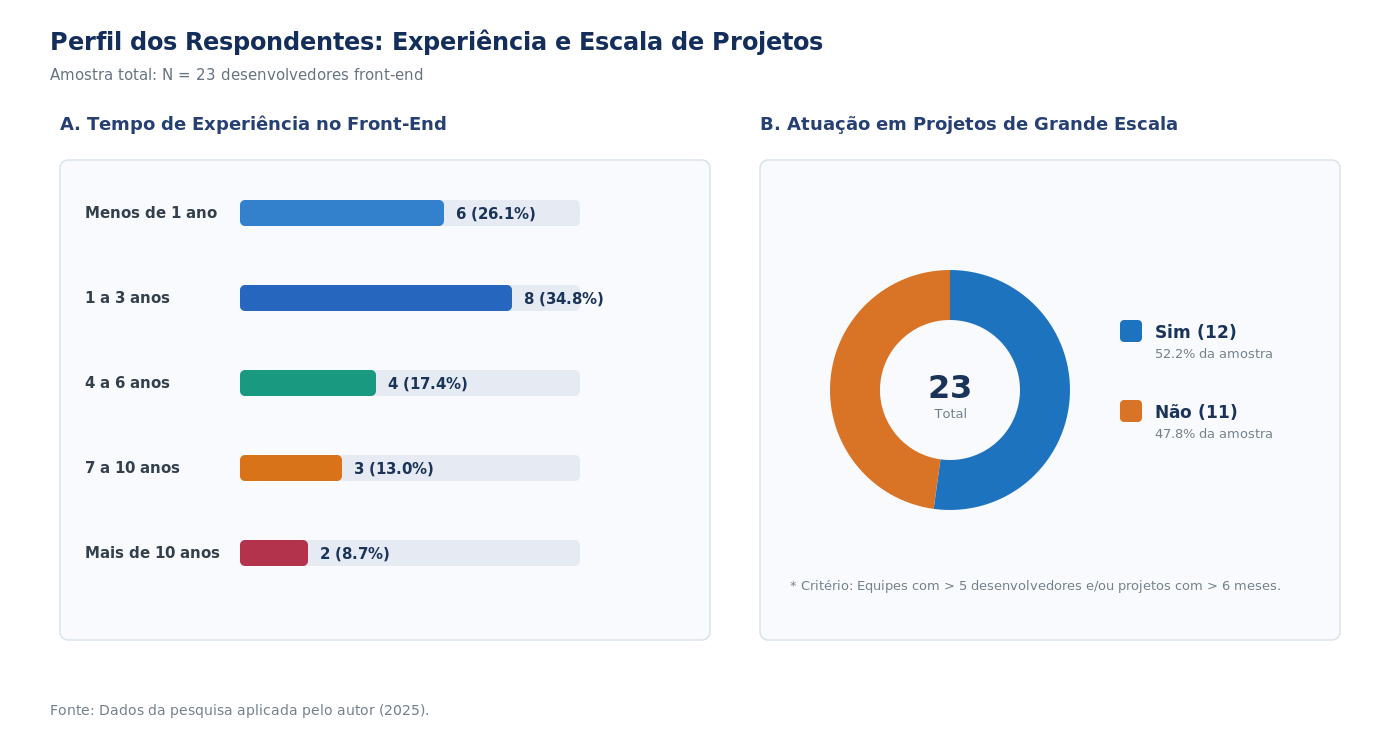
\includegraphics[width=0.95\textwidth]{./04-figuras/fig_demografia_experiencia.png}
    \vspace{0.1cm}
    
    \fonte{Dados da pesquisa aplicada pelo autor (2025).}
\end{figure}

Conforme evidencia a Figura \ref{fig:demografia}(A), os respondentes distribuem-se em diferentes estágios de maturidade na carreira:
\begin{itemize}
    \item \textbf{Menos de 1 ano}: 6 participantes (26,1\%);
    \item \textbf{1 a 3 anos}: 8 participantes (34,8\%);
    \item \textbf{4 a 6 anos}: 4 participantes (17,4\%);
    \item \textbf{7 a 10 anos}: 3 participantes (13,0\%);
    \item \textbf{Mais de 10 anos}: 2 participantes (8,7\%).
\end{itemize}

Para fins de análise comparativa neste estudo, foram estabelecidos dois grupos principais:
\begin{enumerate}
    \item \textbf{Grupo de Desenvolvedores Iniciantes e Intermediários ($N = 14$, 60,9\%)}: composto por profissionais e estudantes em fase de formação com até 3 anos de experiência em desenvolvimento front-end.
    \item \textbf{Grupo de Profissionais Experientes ($N = 9$, 39,1\%)}: formado por participantes com 4 ou mais anos de experiência declarada em desenvolvimento front-end. Neste estudo, ``experiente'' é uma categoria operacional e não equivale necessariamente a um cargo de senioridade.
\end{enumerate}

Adicionalmente, a Figura \ref{fig:demografia}(B) demonstra que 12 participantes (52,2\%) possuem experiência sólida em projetos de grande escala, enquanto 11 participantes (47,8\%) atuaram predominantemente em projetos individuais, de menor porte ou em contexto estritamente acadêmico. Esse equilíbrio amostral é particularmente valioso para avaliar se as dores e os benefícios apregoados pela adoção do TypeScript dependem da escala organizacional do software.

A Figura \ref{fig:proficiencia} apresenta a comparação entre os níveis declarados de proficiência técnica em JavaScript e em TypeScript.

\begin{figure}[H]
    \centering
    \caption{Comparativo de proficiência técnica autoavaliada em JavaScript e TypeScript}
    \label{fig:proficiencia}
    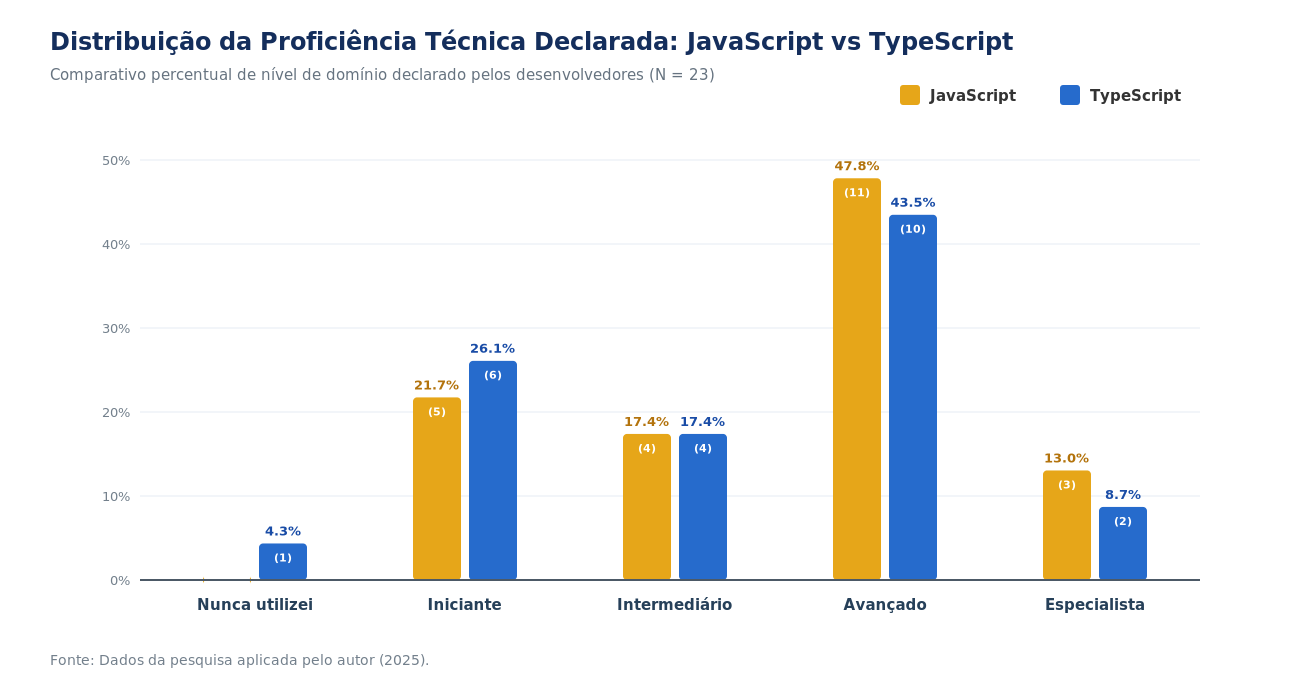
\includegraphics[width=0.92\textwidth]{./04-figuras/fig_nivel_proficiencia.png}
    \vspace{0.1cm}
    
    \fonte{Dados da pesquisa aplicada pelo autor (2025).}
\end{figure}

A autoavaliação de proficiência em JavaScript foi elevada na amostra, com 60,8\% dos participantes posicionando-se nos níveis \textit{Avançado} (47,8\%) ou \textit{Especialista} (13,0\%), e nenhum respondente declarando desconhecimento da linguagem. Em relação ao TypeScript, observa-se uma distribuição similar no topo da escala (52,2\% entre avançados e especialistas), porém com uma fração mais expressiva de iniciantes (26,1\%) e um participante (4,3\%) que declarou nunca ter utilizado a linguagem. Esse panorama é compatível com a literatura que descreve o JavaScript como experiência prévia frequente na aprendizagem do TypeScript \cite{mororo2024}, mas não permite afirmar que essa experiência seja obrigatória.

---

\section{Produtividade e Desenvolvimento Ágil (Bloco A)}
\label{sec:produtividade}

O Bloco A do questionário investigou a percepção dos participantes acerca da velocidade de desenvolvimento, facilidade de prototipagem, curva de aprendizado e detecção de falhas. As respostas foram mensuradas por meio de uma escala Likert de 5 pontos (variando de 1 = Discordo totalmente a 5 = Concordo totalmente).

A Tabela \ref{tab:blocoA} sumariza as métricas estatísticas descritivas (médias, medianas e desvios-padrão) para o conjunto geral da amostra e a desagregação comparativa entre desenvolvedores iniciantes e experientes.

\begin{table}[H]
\centering
\caption{Estatísticas descritivas do Bloco A: Produtividade e Desenvolvimento}
\label{tab:blocoA}
\small
\begin{tabular}{|p{7.5cm}|c|c|c|c|c|c|}
\hline
\rowcolor{gray!20}
\textbf{Item Avaliado} & \textbf{Média} & \textbf{Med.} & \textbf{DP} & \textbf{Inic.} & \textbf{Exp.} & \textbf{$\Delta$ (E-I)} \\
\hline
A1. Desenvolve mais rápido em JS do que em TS & 3,04 & 3,0 & 1,22 & 3,00 & 3,11 & +0,11 \\
\hline
A2. O TS aumenta a produtividade no desenvolvimento & 3,43 & 4,0 & 1,41 & 2,93 & 4,22 & \textbf{+1,29} \\
\hline
A3. A curva de aprendizado do TS é mais íngreme & 3,17 & 3,0 & 1,07 & 2,86 & 3,67 & +0,81 \\
\hline
A4. JS é mais fácil de entender e ensinar a novatos & 4,17 & 4,0 & 0,89 & 4,07 & 4,33 & +0,26 \\
\hline
A5. O TS ajuda a detectar erros mais cedo & 4,17 & 5,0 & 1,19 & 3,79 & 4,78 & \textbf{+0,99} \\
\hline
A6. O JS permite prototipar aplicações mais rápido & 3,83 & 4,0 & 1,23 & 4,29 & 3,11 & \textbf{-1,18} \\
\hline
\end{tabular}
\vspace{0.1cm}

\fonte{Dados da pesquisa aplicada pelo autor (2025).}
\end{table}

A representação gráfica comparativa dessas percepções é ilustrada na Figura \ref{fig:blocoA}.

\begin{figure}[H]
    \centering
    \caption{Comparativo de médias no Bloco A entre Iniciantes e Experientes}
    \label{fig:blocoA}
    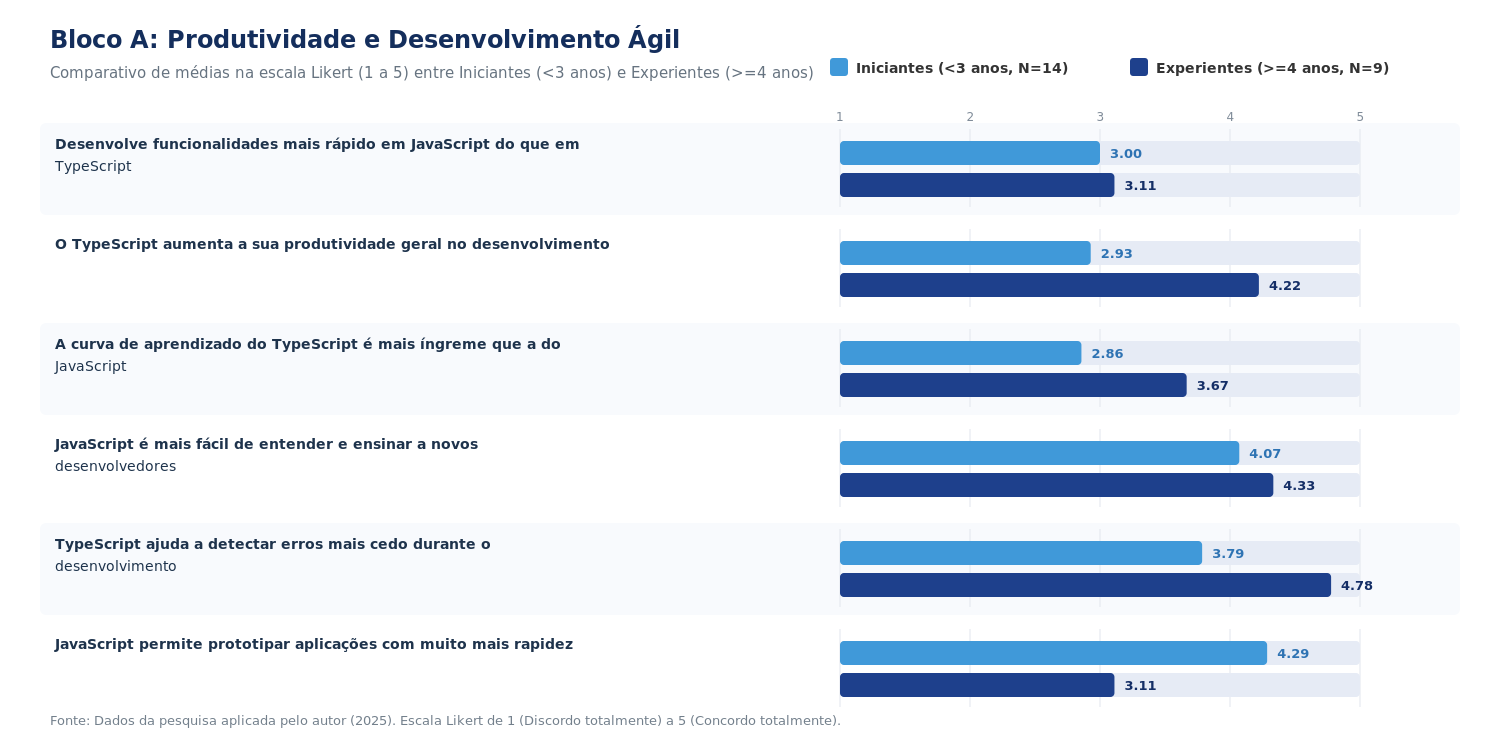
\includegraphics[width=0.98\textwidth]{./04-figuras/fig_blocoA_produtividade.png}
    \vspace{0.1cm}
    
    \fonte{Dados da pesquisa aplicada pelo autor (2025).}
\end{figure}

A análise dos resultados do Bloco A evidencia diferenças associadas ao nível de experiência na percepção de produtividade:

\begin{enumerate}
    \item \textbf{Diferença de percepção de produtividade ($\Delta = +1,29$)}: Enquanto os desenvolvedores iniciantes mantêm uma postura neutra ou reticente quanto aos ganhos de produtividade proporcionados pelo TypeScript (média de $2,93$), os profissionais experientes manifestam maior concordância com essa afirmação (média de $4,22$). Na amostra estudada, essa percepção pode estar relacionada ao uso de autocompletar, refatoração e detecção de inconsistências, mas o desenho da pesquisa não mede produtividade objetiva.
    
    \item \textbf{Prototipagem rápida e flexibilidade ($\Delta = -1,18$)}: O grupo de iniciantes concorda mais fortemente que o JavaScript puro possibilita criar protótipos rapidamente (média de $4,29$), enquanto o grupo experiente apresenta média de $3,11$. Essa diferença é compatível com a percepção de que a configuração inicial do TypeScript pode ser mais custosa, mas não permite concluir que a linguagem seja objetivamente mais lenta em todos os contextos.
    
    \item \textbf{Detecção precoce de erros ($\Delta = +0,99$)}: Ambos os grupos reconhecem o papel do TypeScript na identificação de defeitos antes do envio para produção, com média de $4,78$ e mediana $5,0$ entre experientes. O resultado é compatível com os achados de \cite{richards2017} e \cite{makimov2022}, mas representa percepção dos respondentes, não uma medição direta de defeitos evitados.
    
    \item \textbf{Facilidade Pedagógica}: Tanto iniciantes ($4,07$) quanto experientes ($4,33$) concordam amplamente que o JavaScript é uma linguagem didaticamente mais acessível para a introdução de novos programadores à web, reflexo direto de sua sintaxe não vinculada à tipagem estrita prévia.
\end{enumerate}

---

\section{Qualidade do Código, Manutenibilidade e Prevenção de Falhas (Bloco B)}
\label{sec:qualidade}

O Bloco B concentrou-se na análise das características intrínsecas da base de código: legibilidade, facilidade de manutenção em longo prazo, propensão à geração de defeitos, verbosidade e padronização arquitetural em equipes multidisciplinares.

Os dados estatísticos consolidados do Bloco B estão descritos na Tabela \ref{tab:blocoB}.

\begin{table}[H]
\centering
\caption{Estatísticas descritivas do Bloco B: Qualidade e Manutenção do Código}
\label{tab:blocoB}
\small
\begin{tabular}{|p{7.5cm}|c|c|c|c|c|c|}
\hline
\rowcolor{gray!20}
\textbf{Item Avaliado} & \textbf{Média} & \textbf{Med.} & \textbf{DP} & \textbf{Inic.} & \textbf{Exp.} & \textbf{$\Delta$ (E-I)} \\
\hline
B1. Código em TS é mais legível que em JS & 4,04 & 5,0 & 1,33 & 3,86 & 4,33 & +0,47 \\
\hline
B2. Projetos em TS são mais fáceis de manter a longo prazo & 3,83 & 4,0 & 1,34 & 3,43 & 4,44 & \textbf{+1,01} \\
\hline
B3. JS gera mais bugs por ausência de tipagem & 4,17 & 5,0 & 1,15 & 4,00 & 4,44 & +0,44 \\
\hline
B4. O TS torna o código excessivamente verboso e difícil & 2,39 & 2,0 & 1,16 & 2,57 & 2,11 & -0,46 \\
\hline
B5. TS melhora a padronização em equipes grandes & 4,30 & 5,0 & 0,88 & 4,07 & 4,67 & \textbf{+0,60} \\
\hline
B6. JS facilita soluções rápidas para problemas simples & 4,00 & 4,0 & 1,04 & 4,07 & 3,89 & -0,18 \\
\hline
\end{tabular}
\vspace{0.1cm}

\fonte{Dados da pesquisa aplicada pelo autor (2025).}
\end{table}

A Figura \ref{fig:blocoB} ilustra graficamente o comportamento comparativo das variáveis avaliadas no Bloco B.

\begin{figure}[H]
    \centering
    \caption{Comparativo de médias no Bloco B entre Iniciantes e Experientes}
    \label{fig:blocoB}
    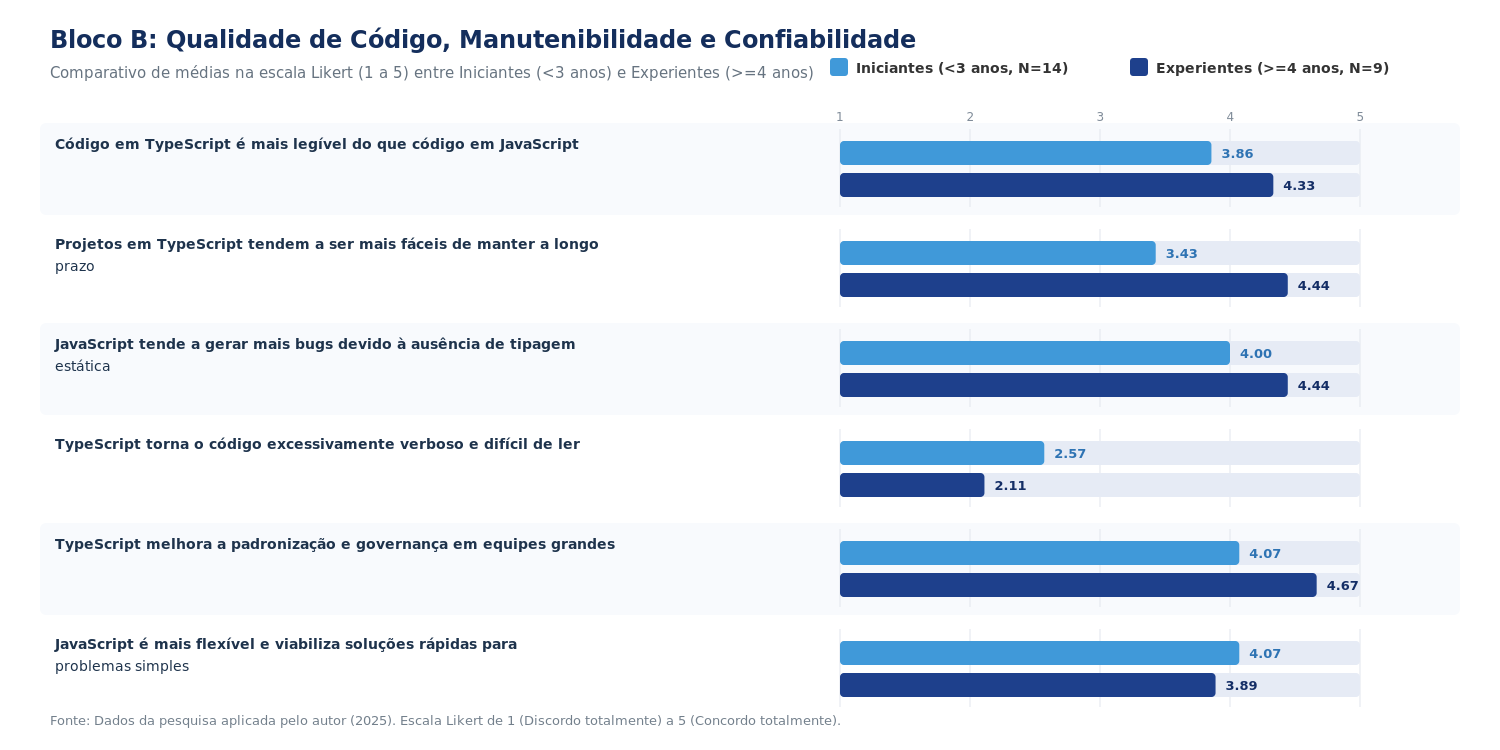
\includegraphics[width=0.98\textwidth]{./04-figuras/fig_blocoB_qualidade_manutencao.png}
    \vspace{0.1cm}
    
    \fonte{Dados da pesquisa aplicada pelo autor (2025).}
\end{figure}

Os resultados do Bloco B reforçam aspectos cruciais da literatura de Engenharia de Software:

\begin{enumerate}
    \item \textbf{Manutenibilidade em longo prazo ($\Delta = +1,01$)}: A assertiva de que bases de código estruturadas em TypeScript são mais sustentáveis recebeu avaliação destacada dos profissionais experientes (média de $4,44$). Ao segmentar a amostra por participação em grandes projetos, a média foi de $4,42$ entre participantes com essa experiência, contra $3,18$ entre os demais. Esses dados sugerem uma associação entre vivência em sistemas maiores e valorização da manutenibilidade, mas não permitem estimar retorno sobre investimento nem afirmar crescimento causal.
    
    \item \textbf{Percepção sobre bugs e tipagem estática}: A afirmação de que a tipagem dinâmica do JavaScript pode favorecer defeitos em tempo de execução obteve alta concordância em ambos os grupos ($4,00$ entre iniciantes e $4,44$ entre experientes; média geral de $4,17$). Esse resultado é compatível com as discussões de \cite{bogner2022} e \cite{george2020}, mas descreve a percepção dos participantes e não uma contagem observada de defeitos.
    
    \item \textbf{Desmistificação da Sobrecarga de Verbosidade}: A hipótese de que o TypeScript tornaria o código excessivamente prolixo ou ilegível foi amplamente rejeitada pelos participantes (média global de $2,39$; $2,11$ entre experientes e $2,00$ entre os atuantes em grandes projetos). Em contrapartida, a legibilidade do código em TypeScript foi avaliada positivamente ($4,04$ geral e $4,33$ para experientes), indicando que os desenvolvedores encaram as anotações de tipo não como ruído, mas como documentação viva acoplada ao código-fonte.
    
    \item \textbf{Governança em Equipes Grandes}: O item que associa o TypeScript ao aprimoramento da padronização e consistência em times numerosos obteve a maior média de todo o bloco ($4,30$ geral e $4,67$ entre experientes, com mediana $5,0$). Esse dado corrobora a tese de que os tipos funcionam como um contrato formal de comunicação interequipes.
\end{enumerate}

---

\section{Compatibilidade, Ferramentas e Desafios de Migração (Bloco C)}
\label{sec:compatibilidade}

O Bloco C investigou a relação do TypeScript com o ferramental moderno de desenvolvimento (IDEs, linters, formatadores), o ecossistema de frameworks de ponta (React, Angular, Vue) e os custos e dificuldades de integrar ou migrar sistemas concebidos originalmente em JavaScript.

A Tabela \ref{tab:blocoC} e a Figura \ref{fig:blocoC} sintetizam as respostas obtidas.

\begin{table}[H]
\centering
\caption{Estatísticas descritivas do Bloco C: Compatibilidade e Ferramentas}
\label{tab:blocoC}
\small
\begin{tabular}{|p{7.5cm}|c|c|c|c|c|c|}
\hline
\rowcolor{gray!20}
\textbf{Item Avaliado} & \textbf{Média} & \textbf{Med.} & \textbf{DP} & \textbf{Inic.} & \textbf{Exp.} & \textbf{$\Delta$ (E-I)} \\
\hline
C1. TS possui excelente suporte em bibliotecas modernas & 4,43 & 5,0 & 0,66 & 4,29 & 4,67 & +0,38 \\
\hline
C2. É fácil migrar/integrar TS em projetos legados JS & 3,61 & 4,0 & 1,12 & 3,86 & 3,22 & \textbf{-0,64} \\
\hline
C3. Ferramentas (IDEs/Linters) suportam melhor o TS & 4,04 & 4,0 & 0,93 & 3,71 & 4,56 & \textbf{+0,85} \\
\hline
C4. JS ainda é mais amplamente suportado & 3,96 & 4,0 & 1,07 & 3,71 & 4,33 & +0,62 \\
\hline
\end{tabular}
\vspace{0.1cm}

\fonte{Dados da pesquisa aplicada pelo autor (2025).}
\end{table}

\begin{figure}[H]
    \centering
    \caption{Comparativo de médias no Bloco C entre Iniciantes e Experientes}
    \label{fig:blocoC}
    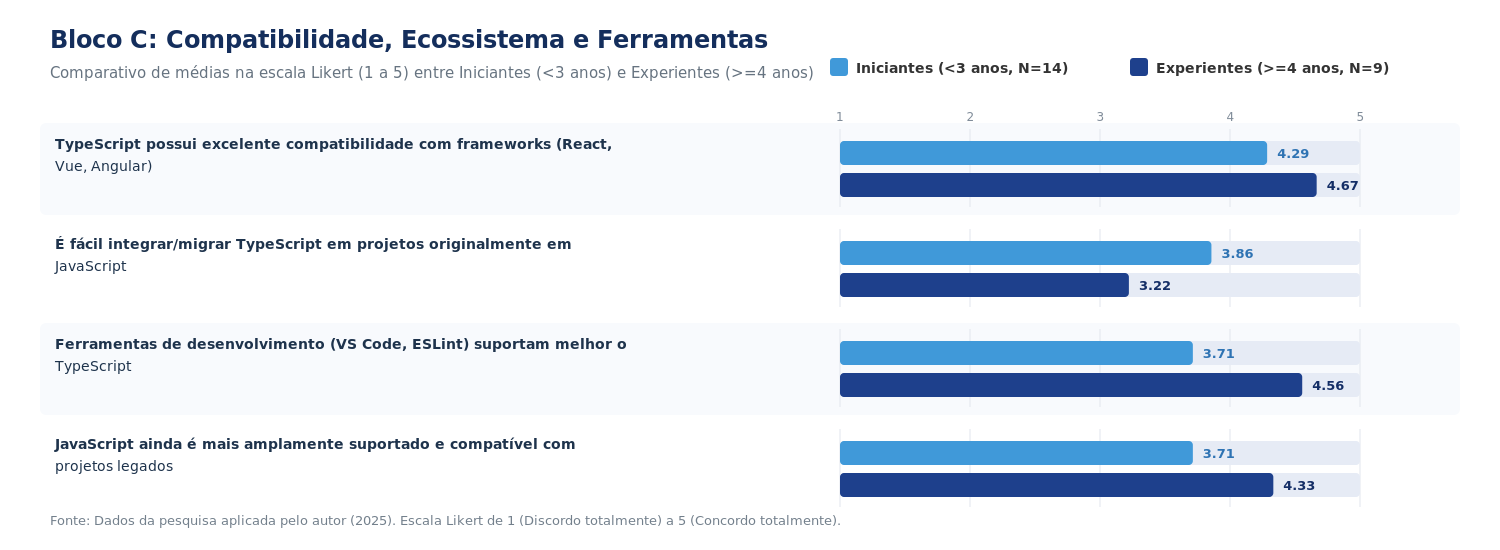
\includegraphics[width=0.98\textwidth]{./04-figuras/fig_blocoC_compatibilidade_ferramentas.png}
    \vspace{0.1cm}
    
    \fonte{Dados da pesquisa aplicada pelo autor (2025).}
\end{figure}

Dentre os principais achados do Bloco C, destacam-se:

\begin{enumerate}
    \item \textbf{Simbiose com o ecossistema e o ferramental ($\Delta = +0,85$)}: O suporte proporcionado por ambientes de desenvolvimento integrados e extensões de análise estática foi avaliado favoravelmente pelos profissionais experientes (média de $4,56$). Na percepção dos respondentes, esses recursos apoiam refatoração, navegação semântica e autocompletar contextual.
    
    \item \textbf{Percepções sobre a migração de projetos legados ($\Delta = -0,64$)}: Os desenvolvedores iniciantes avaliaram o processo de migração de JavaScript para TypeScript como relativamente fácil (média de $3,86$), enquanto os profissionais experientes apresentaram média de $3,22$. A diferença é compatível com a hipótese de que a vivência em bases extensas torna mais visíveis os custos de tipar pacotes de terceiros, gerenciar configurações e refatorar padrões dinâmicos, mas não permite atribuir uma causa única às respostas.
    
    \item \textbf{Compatibilidade com frameworks}: A compatibilidade do TypeScript com frameworks front-end recebeu média de $4,43$ e desvio-padrão de $0,66$. O resultado expressa avaliação favorável dos participantes, mas não permite afirmar, sozinho, que toda a indústria tenha estabelecido um padrão único.
\end{enumerate}

---

\section{Preferências Pessoais, Confiança e Perspectivas Futuras (Bloco D)}
\label{sec:preferencias}

O Bloco D aferiu o vínculo atitudinal e emocional dos desenvolvedores em relação às duas linguagens, mensurando aspectos como nível de confiança psicológica ao codificar, preferência para novos projetos (\textit{greenfield}) e a projeção de relevância futura no mercado.

A Tabela \ref{tab:blocoD} e a Figura \ref{fig:blocoD} detalham as médias apuradas.

\begin{table}[H]
\centering
\caption{Estatísticas descritivas do Bloco D: Preferências e Perspectivas Pessoais}
\label{tab:blocoD}
\small
\begin{tabular}{|p{7.5cm}|c|c|c|c|c|c|}
\hline
\rowcolor{gray!20}
\textbf{Item Avaliado} & \textbf{Média} & \textbf{Med.} & \textbf{DP} & \textbf{Inic.} & \textbf{Exp.} & \textbf{$\Delta$ (E-I)} \\
\hline
D1. Prefiro trabalhar com TS em novos projetos & 3,87 & 4,0 & 1,36 & 3,43 & 4,56 & \textbf{+1,13} \\
\hline
D2. Sinto-me mais seguro e confiante com TS & 3,70 & 4,0 & 1,33 & 3,29 & 4,33 & \textbf{+1,04} \\
\hline
D3. Acredito que o TS será o futuro do front-end & 4,04 & 4,0 & 1,11 & 3,79 & 4,44 & +0,65 \\
\hline
D4. Prefiro JS pela simplicidade e flexibilidade & 2,65 & 3,0 & 1,50 & 3,07 & 2,00 & \textbf{-1,07} \\
\hline
D5. Em equipes grandes, TS traz mais benefícios & 4,22 & 5,0 & 1,00 & 4,00 & 4,56 & +0,56 \\
\hline
\end{tabular}
\vspace{0.1cm}

\fonte{Dados da pesquisa aplicada pelo autor (2025).}
\end{table}

\begin{figure}[H]
    \centering
    \caption{Comparativo de médias no Bloco D entre Iniciantes e Experientes}
    \label{fig:blocoD}
    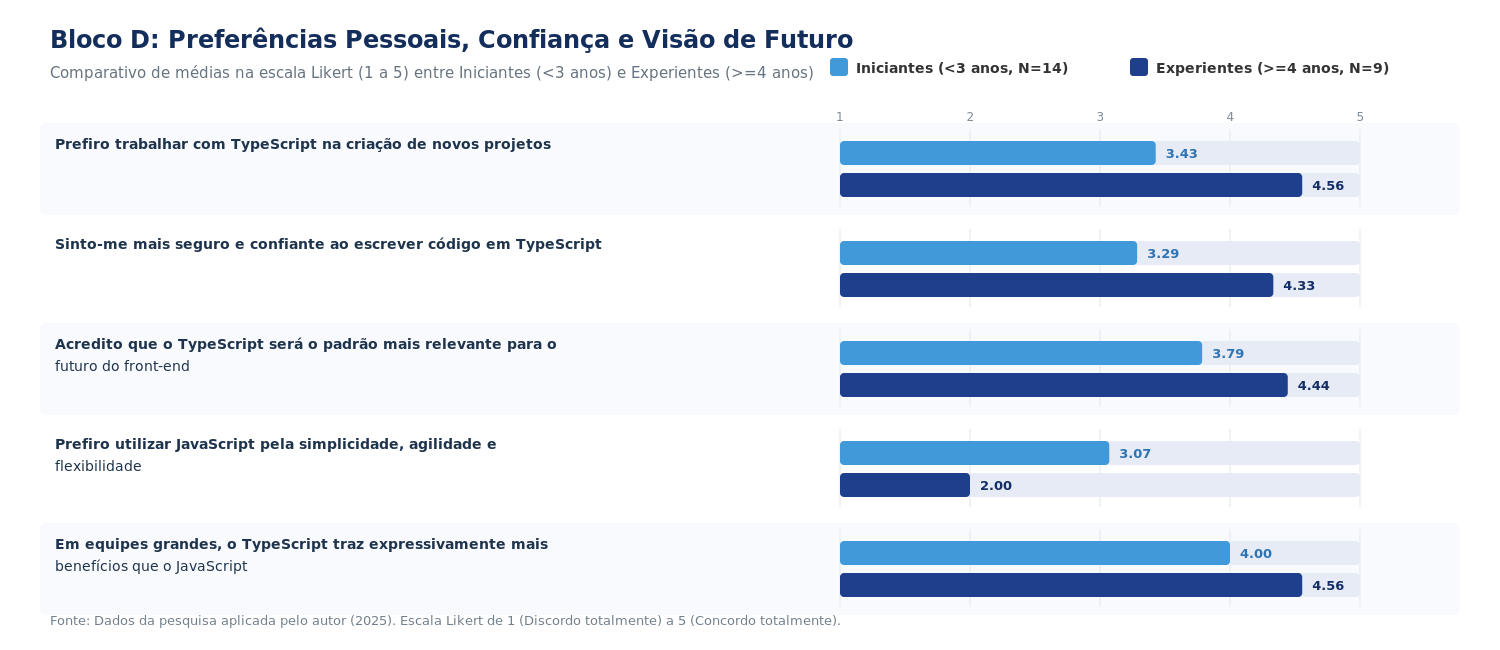
\includegraphics[width=0.98\textwidth]{./04-figuras/fig_blocoD_preferencias_futuro.png}
    \vspace{0.1cm}
    
    \fonte{Dados da pesquisa aplicada pelo autor (2025).}
\end{figure}

A dimensão atitudinal traz revelações expressivas:

\begin{enumerate}
    \item \textbf{Confiança técnica percebida ($\Delta = +1,04$)}: Os desenvolvedores experientes expressam maior confiança ao codificar em TypeScript ($4,33$ contra $3,29$ dos iniciantes). Essa percepção pode estar relacionada ao apoio da validação estática, mas não demonstra, por si só, redução da carga cognitiva ou de erros reais.
    
    \item \textbf{Preferência para novos projetos ($\Delta = +1,13$)}: Diante da oportunidade de iniciar um projeto a partir do zero, os profissionais experientes apresentam maior preferência pelo TypeScript ($4,56$). A preferência pelo JavaScript devido à simplicidade foi menor nesse grupo ($2,00$) do que entre iniciantes ($3,07$), diferença que deve ser interpretada como percepção da amostra.
    
    \item \textbf{Projeção de relevância futura}: Os participantes apresentaram média de $4,04$ para a expectativa de expansão da relevância do TypeScript. Esse resultado descreve uma expectativa da amostra, não uma previsão objetiva do mercado.
\end{enumerate}

A Figura \ref{fig:divergencia} sintetiza as principais divergências perceptuais entre os dois grupos, ordenadas pela magnitude do delta ($\Delta = \text{Média}_{\text{Experientes}} - \text{Média}_{\text{Iniciantes}}$).

\begin{figure}[H]
    \centering
    \caption{Divergência perceptual consolidada entre Experientes e Iniciantes ($\Delta$ de Médias)}
    \label{fig:divergencia}
    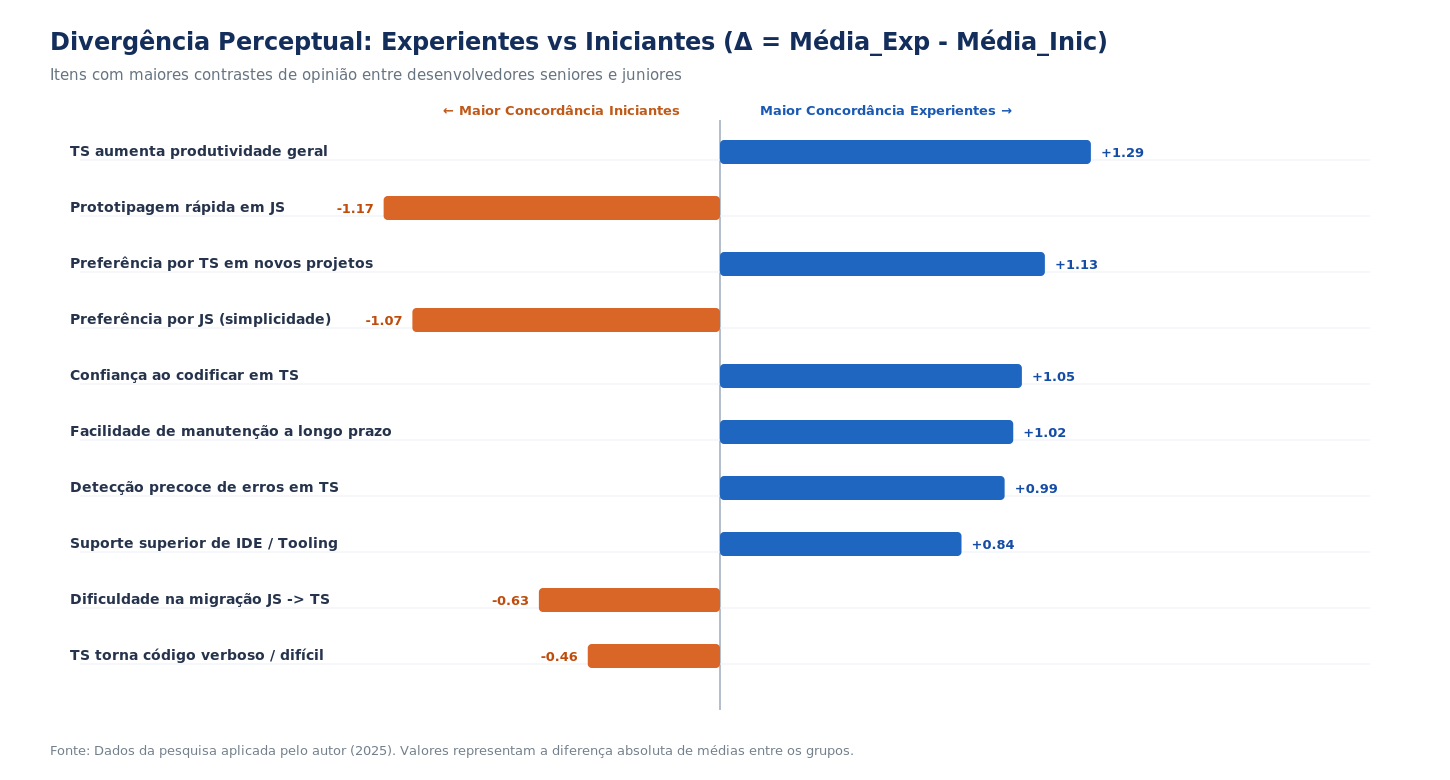
\includegraphics[width=0.98\textwidth]{./04-figuras/fig_comparativo_iniciantes_experientes.png}
    \vspace{0.1cm}
    
    \fonte{Dados da pesquisa aplicada pelo autor (2025).}
\end{figure}

---

\section{Análise Qualitativa dos Relatos Práticos da Indústria}
\label{sec:qualitativa}

A questão aberta final do formulário solicitou aos participantes que relatassem, de forma contextualizada, experiências práticas onde o uso de TypeScript trouxe vantagens tangíveis ou desvantagens operacionais em relação ao JavaScript puro. 

A análise temático-categorial desses depoimentos permitiu consolidar quatro eixos fundamentais que explicam a dinâmica real de adoção na indústria de software:

\subsection{Eixo 1: Blindagem de Contratos de Dados e Integração de APIs}

O benefício mais recorrente citado pelos profissionais foi o estabelecimento de interfaces e contratos estritos na comunicação entre camadas da aplicação e consumo de serviços REST/GraphQL. 

Um desenvolvedor com mais de 10 anos de experiência (Respondente 13) relatou:
\begin{quote}
\textit{``Em projetos Node.js de médio e grande porte, o TypeScript trouxe ganhos significativos de qualidade ao permitir tipagem estática, melhor documentação do código e detecção precoce de erros durante o desenvolvimento. Em especial, em integrações entre múltiplos serviços e APIs, a tipagem ajudou a reduzir falhas de contrato entre componentes e tornou refatorações mais seguras.''} (Respondente 13, Mais de 10 anos de experiência).
\end{quote}

De forma complementar, o Respondente 1 destacou a aplicação em fluxos com regras de negócios críticas:
\begin{quote}
\textit{``Em projetos como o meu livrinho mágico e o portal da motopel o typescript ajudou porque deixou os dados mais seguros por exemplo: ao lidar com usuários, páginas do livro imagens e respostas da api ficaram mais fáceis de evitar erros, que no javascript só apareceriam com o sistema rodando.''} (Respondente 1, 1 a 3 anos de experiência).
\end{quote}

\subsection{Eixo 2: Refatoração em Larga Escala e Propagação de Modificações}

A segurança durante processos de refatoração constitui uma das maiores vantagens operacionais do TypeScript. A existência de tipos algébricos e uniões discriminadas permite que o compilador sinalize automaticamente todos os trechos do sistema que necessitam de adaptação após uma alteração de esquema.

O Respondente 5 (7 a 10 anos de experiência) ilustrou esse mecanismo de forma precisa:
\begin{quote}
\textit{``A atualização de um union type no typescript foi suficiente para gerar erros em todos os pontos que precisavam de atualização no código. Com javascript, seria necessária uma busca manual dos pontos de atualização, já que os erros não seriam manifestados.''} (Respondente 5, Especialista em JS/TS).
\end{quote}

Essa verificação pode reduzir o risco de determinadas regressões silenciosas relacionadas a alterações em modelos de dados centrais, mas não substitui testes, validações de runtime ou revisão da lógica de negócio.

\subsection{Eixo 3: Complexidade Inicial e Fricção com o Ecossistema Externo}

Em contrapartida às vantagens de longo prazo, os relatos analisados apontaram de forma recorrente custos de partida associados ao TypeScript: aumento da complexidade de configuração do ambiente (\textit{toolchain}), esforço inicial para modelar interfaces complexas e atrito com bibliotecas que não disponibilizam definições de tipos adequadas.

O Respondente 12 pontuou essa relação de \textit{trade-off}:
\begin{quote}
\textit{``Em um projeto utilizando Vue.js com Nuxt 3 e TypeScript, trabalhei na implementação de formulários complexos [...]. Houve desvantagens no aumento da complexidade inicial, principalmente ao lidar com tipagens mais avançadas e integração com bibliotecas externas que nem sempre possuem tipagem bem definida, exigindo ajustes manuais ou uso pontual de any. Mesmo assim, o ganho em segurança e escalabilidade compensou o custo inicial.''} (Respondente 12, 4 a 6 anos de experiência).
\end{quote}

Esse relato é compatível com o achado quantitativo de que profissionais experientes reconhecem dificuldades de migração e configuração inicial, embora avaliem favoravelmente os benefícios posteriores de manutenibilidade.

\subsection{Eixo 4: A Fronteira entre Compilação e Execução (Runtime vs Compile-time)}

Um aspecto técnico de extrema relevância, apontado com lucidez pelo Respondente 6, diz respeito à natureza da transpilação do TypeScript e seus limites de proteção:
\begin{quote}
\textit{``TypeScript por apresentar tipagem deixa o codigo muito mais legível e organizado, além de prevenir erros [...]. Porém o TS ele so vai validar e ver errors durante o desenvolvimento, em runtime ele ainda vai aceitar uma String em uma variável declarada como Number, porque por baixo ele vai rodar em JS. então você tem que ficar atento para validar e tratar os dados que está mexendo.''} (Respondente 6, 1 a 3 anos de experiência).
\end{quote}

Essa observação adverte para a falsa sensação de segurança de tipos que o TypeScript pode induzir caso o desenvolvedor presuma que a verificação estática elimina a necessidade de validações em tempo de execução para dados externos, como entradas de formulários e respostas HTTP não confiáveis.

---

\section{Confronto Teórico-Empírico e Síntese da Discussão}
\label{sec:sintese_discussao}

O Quadro \ref{qua:confronto} estabelece a síntese integrativa confrontando as premissas formuladas na literatura com os resultados empíricos apurados nesta pesquisa.

\begin{quadro}[H]
\centering
\caption{Confronto entre a literatura acadêmica e as evidências empíricas da pesquisa}
\label{qua:confronto}
\small
\begin{tabular}{|p{4.2cm}|p{5.0cm}|p{5.5cm}|}
\hline
\rowcolor{gray!20}
\textbf{Dimensão Teórica} & \textbf{Postulado da Literatura} & \textbf{Evidência Empírica da Pesquisa} \\
\hline
\textbf{Prevenção de bugs e robustez} & O sistema de tipos estáticos pode antecipar a identificação de determinados erros \cite{richards2017}. & \textbf{Percepção favorável}. Média global de $4,17$ para a afirmação de que JS gera mais bugs; $4,78$ entre experientes para detecção precoce no TS. \\
\hline
\textbf{Curva de aprendizado e transferência} & O conhecimento prévio em JS pode gerar atrito conceitual na assimilação de TS \cite{shrestha2022}. & \textbf{Compatível}. Iniciantes valorizam a flexibilidade do JS ($4,29$ em prototipagem) e relatam maior custo inicial da tipagem. \\
\hline
\textbf{Qualidade de código versus complexidade} & Aplicações em TS podem apresentar melhor qualidade percebida sem necessariamente reduzir todos os bugs \cite{bogner2022}. & \textbf{Percepção compatível}. Avaliação favorável de legibilidade ($4,04$), padronização ($4,30$) e rejeição da alegação de verbosidade excessiva ($2,39$). \\
\hline
\textbf{Evolução e tendência de mercado} & O suporte de frameworks e ferramentas favorece a adoção de TS \cite{george2020, stackoverflow2023}. & \textbf{Percepção favorável}. Suporte de ecossistema ($4,43$), ferramentas/IDEs ($4,56$ para experientes) e expectativa de relevância futura ($4,04$). \\
\hline
\end{tabular}
\vspace{0.1cm}

\fonte{Elaborado pelo autor (2025).}
\end{quadro}

Em suma, os resultados sugerem que a escolha entre JavaScript e TypeScript não é uma mera disputa estilística, mas uma decisão influenciada pelo horizonte temporal do projeto, pela experiência da equipe e pelas condições de integração. Na amostra analisada, o JavaScript foi associado à prototipagem e à introdução pedagógica, enquanto o TypeScript foi mais valorizado para manutenção, refatoração e coordenação em projetos maiores. Essa evidência não permite afirmar que uma das linguagens seja indispensável em todos os contextos.
